\section{Overall approach}%
\label{approach}

Our goal is to enable private and reliable file exchange between users 
participating in the system, by using their respective devices only.
When Alice and Bob, two users of our system, want to exchange a file \(f\) 
through \name, they start by sharing some information out-of-band, \eg from 
their smartphones.
More precisely, they exchange metadata on \(f\), encryption keys, and
some use-once reply mix-headers.
They use these reply headers to transfer the file contents of \(f\) over a 
network of unreliable nodes while also achieving privacy.

%% Figure~\ref{fig:outline} shows the components needed to obtain the
%% routing information for the headers.  

\begin{figure}[hbt]
  \centering
  \def\svgwidth{0.8\columnwidth}
  %  \import{figures/}{outline_figure_only.pdf_tex}
    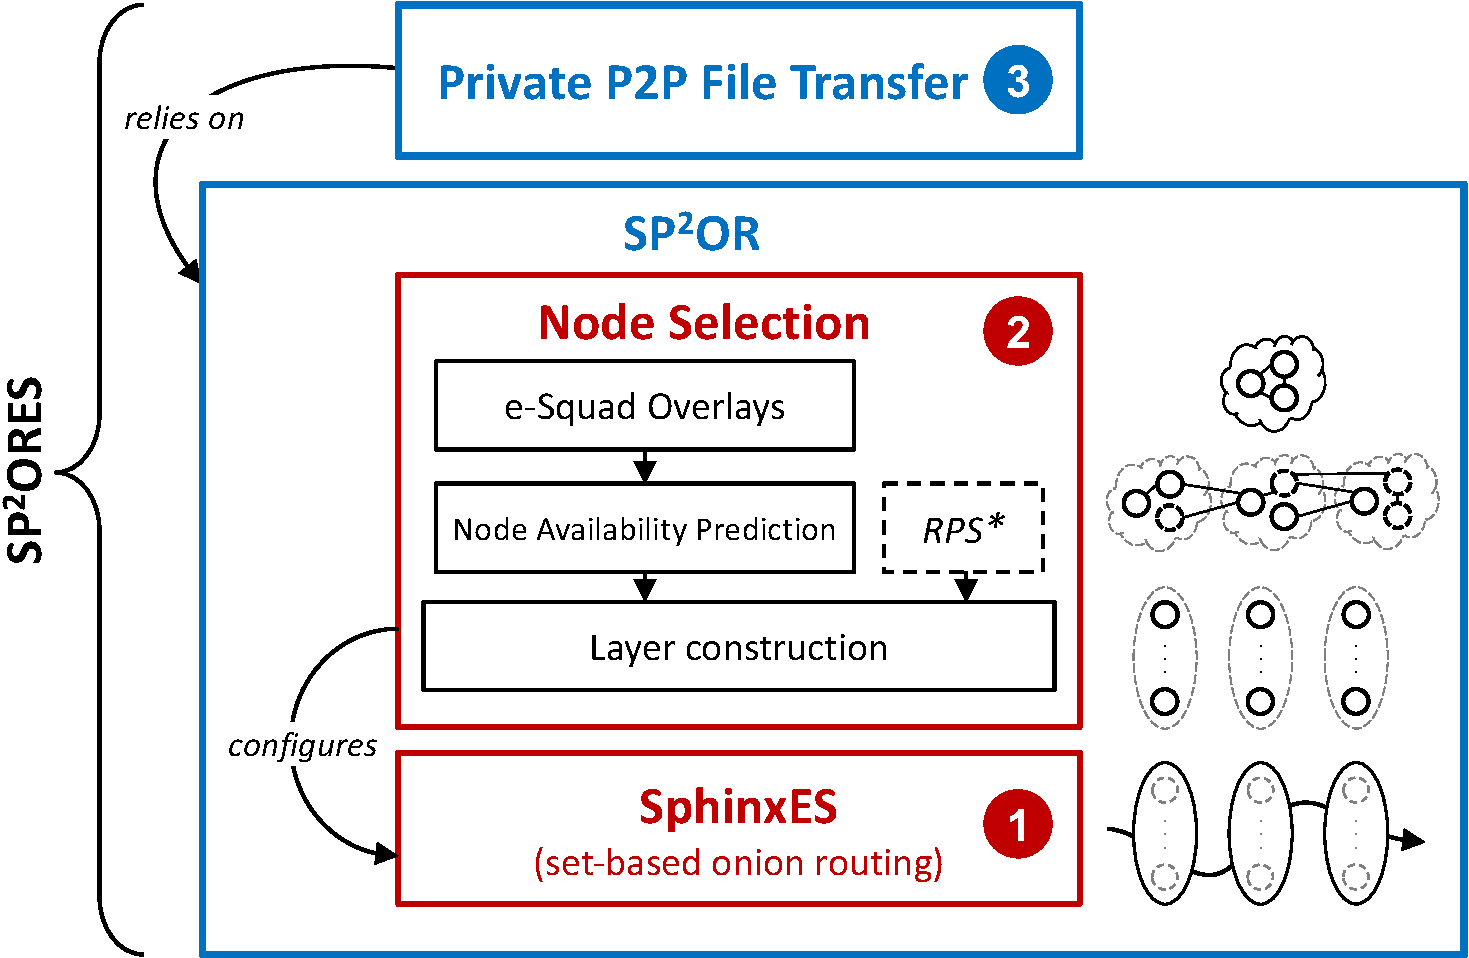
\includegraphics[width=\columnwidth]{figures/OverviewSPORES_cropped}
  \caption{\label{fig:outline}%
    %\commentDaniel{We must adapt this figure to the text.}%
    %% Outline of \name's components. Users' squads of devices are circled in gray. 
    %% From top to bottom: a user's devices collaborate through the Squad Overlay 
    %% (\cref{sec:squad_overlay}); online devices globally share information about 
    %% them with random peers (\cref{ssec:device_availability}); using the two 
    %% overlays above allows for the creation of routes (\ac{SPOR}) between sets of devices. 
    %% These protocols enable secure file transfer between users 
    %% (\cref{ssec:por}).
    \protect\commentFT{TODO by Francois: describe figure}}
\end{figure}

After the initial, out-of-band setup, file transfer happens along
onion routes but with the following features:

\begin{description}
\item [Stateless.] There is no mandatory circuit creation, the file transfer can be
  done in a stateless way. 
\item [Predictive.] The choice of nodes included in the onion routing
  layers is based on a predictive model for availability, disseminated
  by an overlay and queried by random peer sampling.
\item [Probabilistic.] Instead of source routes with one node per onion layer, each
  layer consists of a set of nodes and although the source route still
  determines the sequence of layers, the actual node used for the next
  hop of forwarding is selected from the set in an ad-hoc way,
  resulting in a source-bounded random walk.
\item[Onion Routing.] Put simply, in onion routing, the sender creates
  a source route and 
  encapsulates the payload and next-hop information in layers (by
  encryption), that are \emph{peeled} (decrypted) one by one along the
  route. By virtue of these layers, the forwarding nodes on the
  route do not know where on the route they are and thus whether they
  have received a packet directly from the sender or some other
  intermediate node. We base our format for layering and peeling on
  Sphinx~\cite{Sphinx}, with some modification to allow for the
  changes above, described in \cref{Sphinxes}.
\end{description} 

%\subsection{Taxonomy of anonymous communication protocols}

To present the different parts of \name in detail, 
we align the presentation of the system with the taxonomy of 
\textcite{RoutingSurveyAnonymousProtocols} .
They characterize anonymous communication protocols using the following 
categories (see~\cite[Table 1]{RoutingSurveyAnonymousProtocols}):
\begin{description}
  \item[Network structure.]
    It describes the characteristics of the network nodes, the connections between 
    them and the underlying topology.
    The subcategories are
    \begin{enumerate*}
      \item network topology,
      \item connection type (direction, synchronization),
      \item symmetry (node roles, node topology for routing, decentralization);
    \end{enumerate*}

  \item[Routing information.]
    It describes the network information available to entities deciding on 
    the route of an anonymous file exchange.
    The subcategories are
    \begin{enumerate*}
      \item network view necessary for making routing decisions,
      \item triggers for routing information updates;
    \end{enumerate*}

  \item[Communication model.]
   It describes the entities that make the routing decisions and how they 
    make these decisions.
    The subcategories are
    \begin{enumerate*}
      \item routing type (who selects nodes per route),
      \item scheduling (traffic prioritization),
      \item node selection (determinism, selection set, selection probability);
    \end{enumerate*}

  \item[Performance.]
    It describes things like latency and communication mode.
    The subcategories are
    \begin{enumerate*}
      \item protocol latency,
      \item communication mode (connection- or message-based).
    \end{enumerate*}
\end{description}

We first describe \sphinxes (\cref{Sphinxes}), which is an adaptation of the 

\sonja{do we apply all categories here?}

Sphinx~\cite{Sphinx} mix-header format.
This means that we inherit some properties from Sphinx and due to being only a 
header format, it only imposes some restrictions in the above categories.
\Sphinxes provides, just as Sphinx, unidirectional (network structure), 
message-based (performance) communication.
But unlike Sphinx, \Sphinxes is hybrid source-hop-by-hop routed, a
source-bounded random walk (communication 
model),
\Sphinxes relies on a flat routing-topology (network structure) with fair 
scheduling (communication model) --- as all packets are indistinguishable they 
must be processed on a first-in-first-out basis.
\Sphinxes also introduces some probability to the node selection, but this is 
only a probabilistic selection among already selected nodes and only 
interesting against passive adversaries (an active adversary can learn the 
entire set just as she can learn the single node constituting a layer of a
secure onion-routing scheme without endangering the security
properties~\cite{CLOnionRouting}).

\Sphinxes does \emph{not} introduce any restrictions on whether the network 
topology must be fully connected or not, be asynchronous (as in Tor) or 
synchronous (as in mix-nets), whether node selection must be uniformly random 
or not.
Just as Sphinx, it can be used in many different settings.

Next, we describe the \ac{SPOR} protocol (\cref{SPOR}).
\commentAL{A lot of description here, should only come in Section~\ref{sec:squad_overlay}}
This focuses on the node selection, \ie adds node selection on top of \Sphinxes.
The \ac{SPOR} protocol assumes a source of random nodes, \eg through 
\ac{RPS}~\cite[\eg][]{BrahmsRPS} or \iac{DHT} based 
scheme~\cite[\eg][]{Octopus}.
Each node must be associated with a public key and some availability 
prediction.
\Ac{SPOR} selects nodes for a route uniformly randomly and uses the 
availability to maximize the availability of the entire route, \ie across 
layers.
As \ac{SPOR} assumes this source of random nodes, the network view (routing 
information) of each node depends on this source of random nodes, as does the 
fact of how decentralized the scheme becomes and whether the network toppology 
is fully, mostly or partly connected (network structure).
As \ac{SPOR} is designed, it selects nodes uniformly among all the nodes 
(communication model, node selection) that the source of random nodes provides.
Thus, ultimately, these also depends on the source of random nodes.

A device's availability depends on its user's behavior, hence the device must 
predict this behavior.
This is best done jointly between all of the user's devices.
In \cref{sec:squad_overlay}, we describe a protocol which allows the devices to 
compute their own availability prediction function based on the observations by 
all other devices.

Finally, we describe the complete \ac{SPORES} protocol (\cref{SPORES}), which 
allows the device \squad to act as an autonomous system.
In particular, we introduce a protocol which allows transferring larger 
messages by fragmentation and reassembly across the devices in the \squad.

